\subsection{Business Continuity Process}

Un piano per la continuazione del business si suddivide nei seguenti passi:
\begin{enumerate}
  \item Attuazione dell'\textit{Business Impact Analysis};
  \item Dare priorità ai servizi per supportare i processi critici del 
  business;
  \item Determinazione di modalità alternative di processo per servizi critici
  e vitali;
  \item Sviluppare il piano di \textit{Disaster Recovery} per i servizi di
  recupero IS;
  \item Sviluppo del Business Continuity Plan per le operazioni di recupero e
  continuazione del business;
  \item Test dei piani;
  \item Mantenimento dei piani.
\end{enumerate}

\subsection{Esercizi}

Gli esercizi si trovano nella Sezione \ref{EsBCDR1}.

\section{Disaster recovery testing}

Quando avviene un disastro c'è una persona che ha il compito di allertare le
altre persone (di solito il Chief Security Officer). Quando il CSO dichiara 
l'incidente le persone posso aprire il libro del Disaster Recovery.

Un incidente non viene dichiarato immediatamente, ma c'è una procedura da
rispettare. Quando una situazione di incidente è dichiarata l'incolumità fisica
è la prima a essere presa in considerazione. Gli \textit{Stakeholders} sono
subito contattati, mentre l'ufficio stampa si occupa di dichiarare l'incidente.
Questa parte è molto delicata, e il danno dev'essere spiegato in maniera da non
costituire una brutta pubblicità per l'azienda.

L'ufficio IT entra in azione dopo che tutte queste procedure preliminari sono
annunciate, e comincia ad agire per risolvere il problema.

\subsection{Preparazione di un piano di recupero}

La vita delle persone viene messa sempre in primo piano. Viene poi definito chi
deve fare cosa. Le copie del piano di recupero devono essere distribuite in
diverse locazioni per evitare che possano essere distrutte.

\subsubsection{Preoccupazioni per un piano BCP/DR}

\begin{itemize}
\item Piano d'evacuazione: la vita delle persone è la priorità assoluta;
\item Dichiarazione del disastro;
\item Responsabilità;
\item Procedure per il Disaster Recovery;
\item Procedure per l'Alternate Mode.
\end{itemize}

Copie del piano devono essere mantenute in luoghi secondari.

\subsubsection{Responsabilità in un piano di recupero}

All'interno dell'azienda parte del personale ricopre dei ruoli dal punto di
vista della sicurezza delle persone, e sono pronti ad agire in caso una
situazione di pericolo si manifesti.

Ad esempio, in ogni piano di una struttura (come un ufficio o un edificio
pubblico) dovrebbe essere presente una persona che si incarichi di controllare
ogni stanza per verificare l'assenza di persone in difficoltà in caso di una
evacuazione d'emergenza.

\subsection{Documenti di un piano di recupero}

\begin{table}[H]
\centering
\label{my-label}
\resizebox{\textwidth}{!}{%
\begin{tabular}{|l|p{5cm}|p{5cm}|}
\hline
\textbf{Focus}                   & \textbf{IT}

                                              & \textbf{Business}

                                                                    \\ \hline
Evento di recupero      & Piano di recupero del disastro. Procedure per
recuperare in modalità alternativa   & Piano di recupero del Business. Recupero
del business dopo un disastro                      \\ \hline
                        & Piano di contingenza IT: recupero della maggior parte
delle applicazioni o sistemi & Piano di emergenza per gli occupanti: proteggere
la vita e le risorse sotto pericolo fisico \\ \hline
                        & Piano di risposta per un incidente cibernetico
malizioso                           & Piano di comunicazione di crisi: da un
report della situazione al pubblico e al personale   \\ \hline
Continuità del business &

                            & Piano di continuità del business

                                         \\ \hline
                        &

                            & Piano di continuità delle operazioni in caso di
interruzioni prolungate                     \\ \hline
\end{tabular}%
}
\caption{Lista dei vari documenti di un piano di recupero}
\end{table}

\subsection{Mean Time Between Failure}

Detto anche MTBF, è la somma del \textit{Mean Time to Repair} (MTTR) più il
\textit{Mean Time To Fail} (MTTF), corrisponde al tempo medio che intercorre 
tra l'inizio di due fallimenti.

Il MTTR è il tempo medio necessario per la riparazione, mentre il MTTF è il
tempo medio dalla riparazione ad un nuovo fallimento.

\begin{figure}[H]
 \centering
 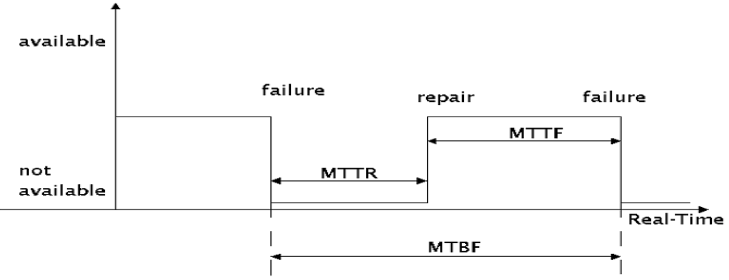
\includegraphics[scale=0.5]{mtbf}
 \caption{Grafico rappresentate i vari valori di un MTBF, MTTR e MTTF}
\end{figure}


L'affidabilità può essere misurata. Un tipica misura è quella detta del
\textit{5 9s}, ovvero del $99.999\%$ di \textit{uptime}, ovvero 5 minuti e
mezzo di fallimento all'anno del servizio.

\subsection{Esecuzione del test}

È l'esecuzione del piano per verificarne il suo funzionamento.
Il test viene effettuato in questo ordine:
\begin{enumerate}
  \item \textbf{Desk-Based Evaluation/Paper test:} un gruppo comincia a 
  seguire i passi della procedura e li esegue a mano, simile al walkthrough;
  \item \textbf{Preparedness Test:} una o più parti dell'intero test vengono
  eseguite personalmente da qualcuno;
  \item \textbf{Full Operational Test:} simulazione di un disastro completo.
\end{enumerate}

\subsubsection{Tipologie di test per la Business Continuity}

Esistono diverse tipologie di test per la \textit{Business Continuity}:
\begin{itemize}
  \item \textbf{Checklist Review:} rivisitazione del piano per verificare
  che tutti gli aspetti importanti siano coperti;
  \item \textbf{Structured Walkthrough:} rivisitazione di tutti gli aspetti
  del piano, spesso guardando tutti gli
  scenari;
  \item \textbf{Simulation Test:} esecuzione del piano basato specificamente 
  per uno scenario, senza un sito alternativo;
  \item \textbf{Parallel Test:} viene azionata la struttura alternativa fuori
  dal sito, senza interrompere il funzionamento del sito regolare;
  \item \textbf{Full-Interruption:} si passa dal sito regolare a quello
  alternativo.
\end{itemize}

\subsubsection{Obiettivi del testing}

L'obiettivo del testing è verificare che il piano riesca a recuperare con
successo le infrastrutture e i processi di \textit{business}.

\paragraph*{Vantaggi} Ci sono i seguenti vantaggi nell'eseguire il testing:
\begin{itemize}
  \item Identificazione di probabili errori;
  \item Verifica delle assunzioni fatte;
  \item Verifica dei tempi;
  \item Allenamento e coordinamento dello staff.
\end{itemize}

\subsubsection{Procedure del testing}

I test sono inizialmente semplici e poi diventano man mano sempre più complessi
con il tempo.

\begin{figure}[H]
 \centering
 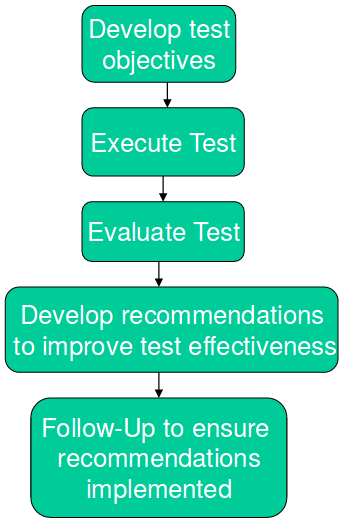
\includegraphics[scale=0.5]{tp}
 \caption{Varie procedure del testing}
\end{figure}

Includono di solito una terza parte indipendente, per poter permetterne una
migliore osservazione.

Dalla valutazione del test si ottengono quelli che sono i \textbf{punti di
miglioramento}, che devono essere effettivamente messi in pratica.

\paragraph*{Passi del test} Esistono diversi passi del test. C'è la sua
preparazione, l'esecuzione del test e la pulizia dopo-test. Importante è
ricordarsi di eseguire una pulizia dei dati dopo l'esecuzione del test, ma di
quelli che non sono importanti per la sua valutazione (altrimenti il test
sarebbe inutile).

\subsubsection{Gap Analysis}

Una \textit{gap analysis} è relativa a un obiettivo che un'azienda si pone
rispetto al punto in cui è, ed è necessaria affinché una azienda possa
migliorare se stessa. Quelli che sono più controllati sono i
processi\footnote{Importante è il PDCA (miglioramento continuo della qualità
dei processi).}, perché le persone sono quelle che sono più difficili da
``modificare'' ed essere migliorate.

\subsection{Auditing di un BCP}

Sono presenti diversi step da controllare, che possono essere:
\begin{itemize}
  \item Include la BIA? La BIA è completa rispetto il RPO/RTO definito per 
  tutti i servizi?
  \item Il BCP in linea con gli obiettivi del business? Sono effettivi e 
  aggiornati?
  \item È chiaro chi deve svolgere cosa nel BCP e nel DRP?
  \item Sono tutti allineati e competenti? Accettano volentieri questo ruolo?
  \item DRP è mantenuto, dettagliato e testato?
  \item Le procedure di backup e di recupero sono seguite?
  \item Il BCP e il DRP sono consistenti con il piano di recupero?
  \item Le persone nella lista del BCP o nell'albero delle chiamate hanno una
  copia del manuale?
  \item L'\textit{hot site} ha tutte le copie del software al momento usato?
  \item Il sito di backup è mantenuto secondo le aspettative? Le 
  aspettative sono effettive?
  \item Il test del DRP è stato documentato per bene? Il DPR è stato 
  aggiornato?
\end{itemize}

\subsubsection{Assicurazione}

Un modo per esternalizzare il rischio completamente è tramite un contratto di
assicurazione.

\begin{figure}[H]
\centering
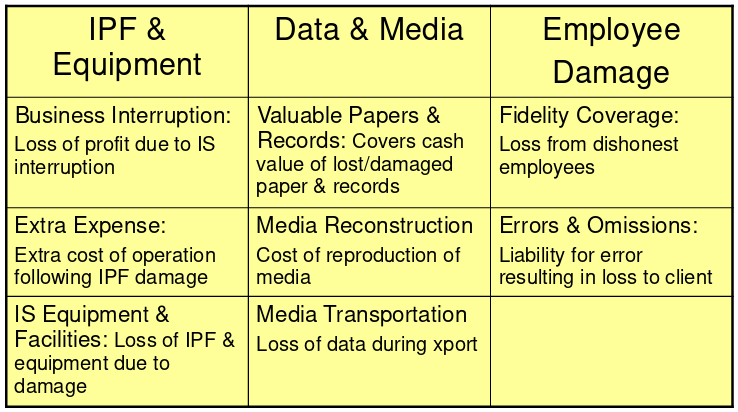
\includegraphics[scale=0.5]{insurance}
\caption[Danni contro i quali ci si può assicurare divisi per
tipologia]{Danni contro i quali ci si può assicurare divisi per
tipologia. La sigla IPF sta per Information Processing Facility
ed è l'edificio che ospita il data center.}
\label{fig:insurance}
\end{figure}


\section{Riassunto dei controlli principali per i controlli di sicurezza BC}

\begin{itemize}
  \item RAID;
  \item Diversi tipi di backup;
  \item Diversi tipi di protezione sulla rete;
  \item Siti alternativi in caso di problemi;
  \item Applicazione di test;
  \item Assicurazione.
\end{itemize}

\section{Esercizi}

Gli esercizi possono essere visti in \ref{EsBCDR2}
